\documentclass[12pt,letterpaper,titlepage,oneside,openright]{book}

\usepackage[utf8]{inputenc}
\usepackage[spanish]{babel}
\usepackage[svgnames]{xcolor}
\usepackage[T1]{fontenc}
% \usepackage[titletoc]{appendix}
\usepackage{amsmath,amsfonts,amsthm}
\usepackage{enumitem}
\usepackage{hyperref}
\usepackage{graphicx}
\usepackage{pdfpages}
\usepackage{lettrine}
\usepackage{listings}
\usepackage{titlesec}
\usepackage{epigraph}
\usepackage{setspace}
\usepackage{fancyhdr}
\usepackage{lipsum}
\usepackage{xspace}
\usepackage{qtree}
\usepackage{color}
\usepackage{tikz}
\usepackage{cite}
\usepackage{anyfontsize}

\fancypagestyle{pagebottom}{
  \renewcommand{\headrulewidth}{0pt}
  \fancyfoot[C]{\thepage}
}

\fancypagestyle{lastpage}{
  \renewcommand{\headrulewidth}{0pt}
  \fancyhead{}
  \fancyfoot{}
}

\makeatletter
\renewcommand{\@chapapp}{}% Not necessary...?
\newenvironment{chapquote}[2][2em]
  {\setlength{\@tempdima}{#1}%
   \def\chapquote@author{#2}%
   \parshape 1 \@tempdima \dimexpr\textwidth-2\@tempdima\relax%
   \itshape}
  {\par\vspace{.5em}\normalfont\hfill--\ \chapquote@author\hspace*{\@tempdima}\par\bigskip}
\makeatother

\setlength{\parskip}{.5em}
\renewcommand{\baselinestretch}{1.2}

\renewcommand{\lstlistlistingname}{Índice de Códigos}
\renewcommand\lstlistingname{Código}
\renewcommand{\spanishlisttablename}{Índice de Tablas}
\renewcommand\spanishtablename{Tabla}

\newcommand{\sat}{\textit{SAT}\xspace}
\newcommand{\sep}{\hspace*{.1em}}

\definecolor{mygray}{gray}{0.8}
\definecolor{pblue}{rgb}{0.13,0.13,1}
\definecolor{pgreen}{rgb}{0,0.5,0}
\definecolor{pred}{rgb}{0.9,0,0}
\definecolor{pgrey}{rgb}{0.46,0.45,0.48}

\titleformat{\chapter} % command
[display] % shape
{\bfseries} % format
{\fontsize{125}{40}\selectfont\textcolor{mygray}{\thechapter}} % label
{-5em} % sep
{
  \Huge\hspace{.5em}
} % before-code
[
  \vspace{1em}%
] % after-code

\lstset{
    basicstyle=\footnotesize\ttfamily,
    commentstyle=\color{pgreen},
    showstringspaces=false,
    keywordstyle=\color{pblue},
    stringstyle=\color{pred},
    rulecolor=\color{black},
    belowskip=\medskipamount,
    frame = trBL,%single,
    framexleftmargin=15pt,
    literate={á}{{\'a}}1 {í}{{\'i}}1 {é}{{\'e}}1 {ó}{{\'o}}1 {ú}{{\'u}}1 {ñ}{{\~n}}1
}

\begin{document}

\frontmatter

\begin{titlepage}
    \begin{center}
        
\includegraphics[width=0.15\textheight]{logo.png}\hspace{1em}
        
\includegraphics[width=0.165\textheight]{ets.png}\\

        \vspace{1em}

        {\large UNIVERSIDAD POLITÉCNICA DE MADRID}\\
        ESCUELA TÉCNICA SUPERIOR DE INGENIEROS INFORMÁTICOS\\
        DEPARTAMENTO DE LENGUAJES Y SISTEMAS INFORMÁTICOS E INGENIERÍA DE SOFTWARE

        \vspace{5.5em}

        \textbf{Parallel SAT solving on a GPU using Zhegalkin polynomial}

        \vspace{5.5em}

        Por:\\
        David Alejandro Lilue Borrero\\
        Con la dirección de:\\
        Julio Mariño\\

        \vfill

        TRABAJO FINAL DE MASTER\\
        Presentado ante la ilustre Universidad Politécnica de Madrid\\
        como requisito para optar al título de Máster en\\
        Software y Sistemas\\

        \vfill
        Madrid, Julio de 2018
    \end{center}
\end{titlepage}

\newpage % Title page
\cleardoublepage
\phantomsection
\addcontentsline{toc}{chapter}{Dedicatoria}
\begin{flushright}
Para todas esas personas\\
que han hecho sentir a un desconocido como en casa,\\
donde la curiosidad y tolerancia superan los miedos,\\
y de alguna forma, mágica, nace la hermandad.
\end{flushright}

\newpage
\cleardoublepage
\phantomsection
\addcontentsline{toc}{chapter}{Agradecimientos}
\begin{flushleft}
Agradezco a ese avión de papel\\
que le ha permitido volar al kiwi\\
dejando en su camino una estala con forma de espiral,\\
aquella posee una proporción casi divina; de oro.
\end{flushleft}

\newpage
\cleardoublepage
\phantomsection
\addcontentsline{toc}{chapter}{Resumen}
\thispagestyle{pagebottom}
\noindent\textbf{\Huge Resumen}

\vspace{2em}

El problema \sat tiene como objetivo determinar si existe una posible combinación de valores que satisfaga una proposición booleana. Dicho problema fue el primero que se demostró ser NP-completo, no existe un algoritmo que solucione este problema de forma eficiente, es decir, en tiempo polinomial. Por otro lado, tenemos los problemas \textit{CSP}, que determinan si un conjunto finito de restricciones con un número específico de variables puede llegar a ser satisfactible, estos problemas pueden ser interpretados y reducidos a \sat. Esto nos lleva a enfocarnos en este problema tan famoso, ya que tiene el poder de aproximar distintos problemas traduciendo las condiciones a fórmulas lógicas.

En la actualidad, y desde hace unos años, los algoritmos para resolver \sat están divididos en dos clases: algoritmos \textit{conflict-driven clause learning}, basados en \textit{DPLL}, y de busqueda local probabilística. Ambas tienen diferentes \textit{solvers} que implementan los algoritmos, algunos usando paralelismo, como \textit{ManySAT}. Estos algoritmos requieren conventir las fórmulas proposicionales en su, equivalente, forma normal conjuntiva (\textit{CNF}), permitiendo separar la fórmula en clausulas que faciliten la comprobación de su satisfacibilidad. Otras representaciones pueden brindar un enfoque diferente, y dependiendo del caso, estas podrían adaptarse mejor a casos específicos; así como los diagramas de desición binaria (\textit{BDD}).

Esto nos motiva a usar una representación diferente y que permita tener un nuevo acercamiento a \sat. El polinomio de \textit{Zhegalkin} nos permite tener un nuevo punto de vista y su forma nos impulsa a buscar una implementación que tenga una estrategia basada en paralelismo usando recursos de la \textit{GPU}. Esta representación nos permite convertir una fórmula lógica a un polinomio en donde las variables pueden tomar valores binarios y, aprovechando esa estructura, se pueden incorporar tácticas de paralelismo usadas para polinomios con el objetivo de buscar una nueva solución a \sat.

\newpage
\cleardoublepage
\phantomsection
\addcontentsline{toc}{chapter}{Abstract}
\thispagestyle{pagebottom}
\noindent\textbf{\Huge Abstract}

\vspace{2em}

The \sat problem intends to determine if there is a possible permutation of values which satisfies a boolean proposition. This problem was the first in being prove to be NP-complete, there is no algorithm such gives a solution to this problem in an efficient way, i.e. polynomial time. On the other hand, we have the CSP problems, these checks if a finite number of constraints, with a specific number of variables, can be satisfy. This problems can be interpreted and reduced to \sat. Given this, we are focusing on this famous problem, since it has the power to embrace different problems, translating the conditions into logical formulas.

Currently, and since a few years, \sat solvers implements two kinds of algorithm, which are these: conflict-driven clause learning algorithm, based in DPLL, and stochastics local searchs. Both have many implementations, some are famous \sat solvers, other use a paralell strategy like \textit{ManySAT}. These algorithms need to rewrite the propositional formula into its conjunctive normal form (CNF), allowing to split the formula in clauses which ease the tests of satisfiability. Other formula representations could bring a different approach, and in some cases, they perform better. For example, the binary decision diagrams (BDD).

All this give us the motivation to use a different representation of boolean propositions, letting us have a new approach to \sat. The \textit{Zhegalkin} polynomial allow us to have a new point of view and its shape brings up the possibility to use parallelism in the implementation, using GPU resources. This representation allow us to convert a boolean proposition into a polynomial, where the variables take binary values. Taking advantage of its structure, similar to normal polynomials, it is possible to use parallel method with little variations, aiming to find a new solution to \sat.

\newpage

{\setstretch{1.0}\setlength{\parskip}{0.6em}
  \tableofcontents
  \listoffigures
  \listoftables
}

\newpage

\mainmatter

\chapter{Introducción}

\begin{chapquote}{Miguel de Cervantes, \textit{Don Quijote de la Mancha}}
Sola una cosa tiene mala el sueño, según he oído decir, y es que se parece a la muerte, pues de un dormido a un muerto hay muy poca diferencia.
\end{chapquote}

Viendo el enfoque actual que se le ha dado al problema \sat, y su capacidad para adaptarse a distintos escenarios, motiva a buscar cualquier mejora o aceleramineto en un algoritmo que lo resuelva. Este problema ha sido ampliamente estudiado, siguiendo una misma linea que en el presente ha alcanzado buenas implementaciones de una solución. Aunque, existe la posibilidad de explorar una visión alternativa, y esta permita abrir una puerta a nuevas soluciones.

Muchos problemas pueden expresarse como proposiciones lógicas, como los problemas de satisfacción de restricciones (\textit{CSP}), y eso permite abarcar una area mayor de impacto en el caso de realizar avances científicos cuando se busca una solución a \sat. Actualmente las soluciones están centradas en la forma normal conjuntiva (\textit{CNF}) de una proposición booleana, esto se debe a que permite descartar facilmente una asignación de valores (\textit{TRUE} o \textit{FALSE}) para las variables involucradas en la fórmula lógica. Esta representación separa las proposiciones en cláusulas, si alguna de ellas no se cumple, se puede descartar el resto de ellas. Por otro lado, las implementaciones actuales tienen enfoques diferentes, algunas secuenciales, otras en paralelo y también exiten otras más probabilísticas pero manteniendo la misma representación.

En ciertos casos, se puede ver una representación como los diagramas binarios de desición (\textit{BDDs}) para resolver \sat, esta puede tener ventajas en ciertos aspectos, u ocasiones, pero sigue sin tener el impacto que tiene \textit{CNF}. Hay implementaciones que usan paralelismo para solucionar \sat pero este tipo de estrategias tienden a ser más dificiles de implementar para estructuras arborescentes como los \textit{BDDs}. Por lo tanto, el objetivo es encontrar una representación que pueda brindar un nuevo enfoque a \sat y que tenga la versatilidad para tener implementaciones en paralelo.

El polinomio de \textit{Zhegalkin} es una representación para proposiciones booleanas, basada en los polinomios usuales en algebra, esta traduce los operadores lógicas de conjunción ($\land$), disyunción ($\lor$), implicación ($\implies$), equivalencia ($\iff$) y negación o complemento ($\neg$), a un polinomio que solo posee dos operadores, conjunción ($\cdot$) y disyunción exclusiva ($\oplus$). Una ventaja de esta representación es que solo la existencia de un polinomio para una fórmula lógica implica su satisfactibilidad. Otro aspecto importante es la posibilidad de implementar una solución que opere en paralelo, ya que los polinomios tienen una estructura propicia para separarse en tareas que pueden delegarse.

\section{\textit{CSP}}

Los problemas de satisfacción de restricciones (\textit{CSP}) son preguntas formuladas a partir de un conjunto de objectos cuyo estado está definido por un número finito de limitaciones. Algunos de estos problemas son conocidos, por ejemplo un sudoku, crucigrama, coloración de grafos, el problema de las ocho reinas, entre otros. Todos ellos son traducibles a \sat, un ejemplo de ello se puede ver en las figuras \ref{fig:g_col_csp} y \ref{fig:g_col_sat}, donde se muestra el mismo problema de coloración del grafo en la figura \ref{fig:graph} modelado de forma diferente.

En la figura \ref{fig:g_col_sat} se construye una proposición lógica siguiendo una notación para el nombre de las variables donde la primera letra es el nodo en minúsculas y la segunda es el color, por ejemplo \textit{ar} es el nodo \textit{A} de color rojo. Solo se muestra el nodo \textit{A} pero sigue el mismo patrón para los otros nodos.

\begin{figure}
\centering
\begin{minipage}{0.5\textwidth}
\begin{tikzpicture}
  [scale=.8,auto=left,every node/.style={circle,fill=blue!20}]
  \node (n1) at (2,4) {A};
  \node (n2) at (4,7) {B};
  \node (n3) at (4,1) {C};
  \node (n4) at (7,7) {D};
  \node (n5) at (7,1) {E};
  \node (n6) at (9,4) {F};

  \draw (n1) -- (n2);
  \draw (n1) -- (n2);
  \draw (n1) -- (n3);
  \draw (n1) -- (n4);
  \draw (n1) -- (n5);

  \draw (n2) -- (n3);
  \draw (n2) -- (n4);
  \draw (n2) -- (n6);

  \draw (n3) -- (n5);
  \draw (n3) -- (n6);

  \draw (n4) -- (n5);
  \draw (n4) -- (n6);

  \draw (n5) -- (n6);
\end{tikzpicture}
\caption{Grafo sin colorear}
\label{fig:graph}
\end{minipage}\hfill
\begin{minipage}{0.5\textwidth}
\begin{tikzpicture}
  [scale=.8,auto=left,every node/.style={circle}]
  \node[fill=red!80] (n1) at (2,4) {A};
  \node[fill=green!80] (n2) at (4,7) {B};
  \node[fill=blue!80] (n3) at (4,1) {C};
  \node[fill=blue!80] (n4) at (7,7) {D};
  \node[fill=green!80] (n5) at (7,1) {E};
  \node[fill=red!80] (n6) at (9,4) {F};

  \draw (n1) -- (n2);
  \draw (n1) -- (n2);
  \draw (n1) -- (n3);
  \draw (n1) -- (n4);
  \draw (n1) -- (n5);

  \draw (n2) -- (n3);
  \draw (n2) -- (n4);
  \draw (n2) -- (n6);

  \draw (n3) -- (n5);
  \draw (n3) -- (n6);

  \draw (n4) -- (n5);
  \draw (n4) -- (n6);

  \draw (n5) -- (n6);
\end{tikzpicture}
\caption{Grafo coloreado}
\label{fig:graph_color}
\end{minipage}
\end{figure}

\begin{figure}
\begin{align*}
    & A, B, C, D, E, F \in \{Red,\ Green,\ Blue\}\\
    \\
    & A \neq B \land A \neq C \land A \neq D \land A \neq E\\
    & B \neq C \land B \neq D \land B \neq E \land B \neq F\\
    & C \neq E \land C \neq F\\
    & D \neq E \land D \neq F\\
    & E \neq F
\end{align*}
\caption{Restricciones para la coloración del grafo}
\label{fig:g_col_csp}
\end{figure}

\begin{figure}
\begin{align*}
    (ar \lor ag \lor ab)\ \land\\
    \neg(ar \land ag)\ \land \neg(ar \land ab)\ \land \neg(ag \land ab)\ \land\\
    \neg(ar \land br)\ \land \neg(ar \land cr)\ \land \neg(ar \land dr)\ \land \neg(ar \land er)\ \land\\
    \neg(ag \land bg)\ \land \neg(ag \land cg)\ \land \neg(ag \land dg)\ \land \neg(ag \land eg)\ \land\\
    \neg(ab \land bb)\ \land \neg(ab \land cb)\ \land \neg(ab \land db)\ \land \neg(ab \land eb)\ \land\\
    \vdots
\end{align*}
\caption{Restricciones para la coloración del grafo en \sat}
\label{fig:g_col_sat}
\end{figure}

\section{Estructura del trabajo}

En los siguientes capítulos se describirá el proceso de implementación a una solución a \sat, comenzando por definir detalladamente esta representación junto a las implementaciones que se desarrollaron. Siguiendo con el diseño de una implementación que aproveche los recursos de la \textit{GPU}, a través de la plataforma OpenCL. Es importante resaltar, que para este trabajo trabajo se ha usado la versión \texttt{1.2}; en todo momento que se refiera a esta plataforma, la versión es tácita. También se describen otros soluciones que se implementaron, seguidas de los resultados experimentales obtenidos y un breve análisis de los mismos. Finalizando con las conclusiones y posibles trabajos futuros.

\chapter{Otras implementaciones}

\begin{chapquote}{Emile Michel Cioran, \textit{Silogismos de la amargura}}
Sólo los espíritus agrietados poseen aberturas al más allá.
\end{chapquote}

Adicionalmente a la implementación del polinomio de \textit{Zhegalkin}, se ha elaborado un prototipo en \textit{Haskell} del algoritmo \textit{DPLL}, usando la representación \textit{CNF} y otro para la conversión de fórmulas proposicionales a \textit{BDDs}. Esto con el objetivo de tener una prueba conceptual de soluciones que existen actualmente para \sat.

\section{\textit{CNF}}

Esta representación separa a una fórmula lógica en cláusulas operadas por la operación ($\land$), reduciendo el problema \sat a buscar la cláusula que no se cumpla dada cierta asignación de valores booleanos a las variables. Es evidente que se irían verificando las cláusulas hasta que alguna falle, en ese momento se sabría que esa permutación de valores para la proposición no es satisfactible. El proceso de normalización comienza obteniendo la forma normal negativa de la proposición lógica para luego aplicar la propiedad distributiva del ($\lor$) sobre ($\land$) hasta que no se pueda aplicar más. El algoritmo \textit{DPLL}, que está basado en el comportamiento de \textit{CNF}, se enuncia a continuación.

\subsection{\textit{DPLL}}

El algortimo \textit{Davis–Putnam–Logemann–Loveland} (\textit{DPLL}) realiza una busqueda usando \textit{backtracking}, donde en cada paso hay una toma de desición y comprobación de las cláusulas que conforman a la proposición lógica. La implementación en \textit{Haskell} reside en una función que se llama recursivamente tomando una desición en cada paso y aporvecha la evaluación perezosa para dividir desiciones de asignación binaria en una simple disyunción.

\section{\textit{BDDs}}

Los diagramas binarios de desición (\textit{BDDs}) es una representación útil porque resulta ser incremental, se pueden operar entre ellos y reproducir un nuevo \textit{BDD}, el cual tendrá las restricciones de ambos dependiendo del operador que se haya usado; manteniendo orden y unicidad. Comportamiento compartido con el polinomio de \textit{Zhegalkin}. Los \textit{BDDs} pueden tener muchas utilidades, ya que indican facilmente si una proposición lógica se satisface o no, asi como los valores necesarios para que se satisfga. Pero en lo que se refiere a \sat, resulta costoso mantener una estructura arborescente ordenada y dado que el objetivo es paralelizar procesos, no se consideró oportuno como una opción para implementar con OpenCL.

\chapter{Polinomio de \textit{Zhegalkin}}

\begin{chapquote}{Rudyard Kipling, \textit{El gato que caminaba solo}}
Eres el Gato que camina solo y a quien no le importa estar aquí o allá. No eres un amigo ni un servidor. Tú mismo lo has dicho. Márchate y camina solo por cualquier lugar.
\end{chapquote}

En este capítulo se expondrá una forma poco usual de expresar formulas lógicas, en lo que se refiere a la resolución del problema \sat, así como su representación abstracta al momento de implementar el \textit{solver} dependiendo del lenguaje de programación. Para este trabajo se ha usado \textit{Haskell} para elaborar un prototipo funcional y, a fin de usar los recursos de la tarjeta gráfica, se usa el lenguaje \textit{C} por su compatibilidad con la librería \textit{open source} OpenCL. En primer lugar se esbozan los conceptos esenciales, siguiendo la implementación funcional, para luego profundizar en la implementación secuencial imperativa.
En este capítulo se expondrá una forma poco usual de expresar formulas lógicas, en lo que se refiere a la resolución del problema \sat, así como su representación abstracta al momento de implementar el \textit{solver} dependiendo del lenguaje de programación. Para este trabajo se ha usado \textit{Haskell} para elaborar un prototipo funcional y, a fin de usar los recursos de la tarjeta gráfica, se usa el lenguaje \textit{C} por su compatibilidad con la librería \textit{open source} OpenCL. En primer lugar se esbozan los conceptos esenciales, siguiendo la implementación funcional, para luego profundizar en la implementación secuencial imperativa.

\section{Definición}

\emph{Ivan Ivanovich Zhegalkin} introdujo en 1927 una forma de representar operaciones en álgebra booleana. El polinomio de \textit{Zhegalkin}, conocido también con el nombre de \textbf{forma normal algebraica} (\textit{ANF}), está constituida por un número finito de monomios operados por la operación \textit{XOR} ($\oplus$), estos se conforman por la multiplicación ($\cdot$) de variables que pueden tomar los valores $0$ o $1$; siendo estos valores posibles monomios. Además, no se permite expresar el complemento de una variable o monomio.

\subsection{Propiedades de los operadores}

Es importante enunciar ciertas propiedades que ilustran el comportamiento de esta representación. Además de ser útiles, y necesarias, al momento de implementar una solución, se usan para reducir los polinomios y mantener la forma normal algebraica.

\begin{figure}[!ht]
\[1 \cdot P \equiv P\]
\caption{Identidad de ($\cdot$)}
\end{figure}

\begin{figure}[!ht]
\[0 \oplus P \equiv P\]
\caption{Identidad de ($\oplus$)}
\end{figure}

\begin{figure}[!ht]
\[0 \cdot P \equiv 0\]
\caption{Elemento absorbente de ($\cdot$)}
\end{figure}

\begin{figure}[!ht]
\[P \cdot P \equiv P\]
\caption{Idempotencia de ($\cdot$)}
\end{figure}

\begin{figure}[!ht]
\[P \oplus P \equiv 0\]
\caption{Eliminación de monomios iguales por ($\oplus$)}
\label{fig:oplus_e}
\end{figure}

No queda de más decir que el operador ($\cdot$) tiene mayor precedencia que ($\oplus$). Por otro lado, los polinomios de \textit{Zhegalkin} cumplen con la propiedad distributiva, de igual forma que los polinomios usuales en algebra. Así como las propiedades conmutativas para ($\cdot$) y ($\oplus$).

\subsection{Equivalencia con operaciones lógicas}

Existe una correspondencia entre las operaciones booleanas ($\land$), ($\lor$), ($\implies$), ($\iff$) y ($\neg$), y las operaciones ($\oplus$) y ($\cdot$). A continuación, en la tabla \ref{table:1}, se presenta cada operación con su respectiva equivalencia.

\begin{table}[h!]
\centering
\begin{tabular}{|| c | c ||}
 \hline
 Operación Booleana & Equivalente \textit{ANF} \\ [0.1ex]
 \hline\hline
 $P \land Q$ & $P\cdot Q$  \\
 $P \lor Q$ & $P\oplus Q\oplus P\cdot Q$  \\
 $P \implies Q$ & $1\oplus P\oplus P\cdot Q$  \\
 $P \iff Q$ & $1\oplus P\oplus Q$  \\
 $\neg P$ & $1\oplus P$  \\
 \hline
\end{tabular}
\caption{Tabla de equivalencia entre operaciones}
\label{table:1}
\end{table}

Se puede deducir el caso de $P \iff Q$ traduciendo a ${P\implies Q \land Q \implies P}$, aplicando la propiedad distributiva de ($\cdot$) sobre ($\oplus$) y reduciendo el polinomio, como puede verse a continuación.

\begin{figure}
\begin{align*}
                 & P\implies Q\land Q \implies P\\
    \rightarrow\ & (1\oplus P\oplus P\cdot Q)\land (1\oplus Q\oplus P\cdot Q)\\
    \rightarrow\ & (1\oplus P\oplus P\cdot Q)\cdot (1\oplus Q\oplus P\cdot Q)\\
    \rightarrow\ & 1\oplus P\oplus P\cdot Q \oplus Q\oplus P\cdot Q\oplus P\cdot Q \oplus P\cdot Q \oplus P\cdot Q \oplus P\cdot Q\\
    \rightarrow\ & 1\oplus P\oplus Q
\end{align*}
\caption{Conversión de la equivalencia a polinomio}
\label{fig:equiv}
\end{figure}

\section{Implementación en \textit{Haskell}}

En principio es necesario poder representar proposiciones lógicas y construir a partir de restricciones, que establezca un problema determinado, con el fin de poder modelar mediante una fórmula proposicional. Para ello, se diseñó un tipo de dato abstracto arborescente (recursivo), que permite representar formulas lógicas. A continuación, en la figura \ref{fig:mp}, se puede ver un ejemplo para ilustrar la idea que se plantea.

\begin{figure}[!ht]
    \Tree [.$\implies$ [.$\land$ [.$\implies$ P Q ] P ] Q ]
\caption{Modus Ponens}
\label{fig:mp}
\end{figure}

\subsection{De proposición lógica a polinomio de \textit{Zhegalkin}}
\label{sec:fromProp}

Para construir el polinomio de \textit{Zhegalkin} a partir de una formula proposicional, se usa la equivalencia de la tabla \ref{table:1} mientras se recorre recursivamente la estructura arborescente y aplicando las distintas propiedades. Si se logra contruir un polinomio que no esté vacío, se puede decir que la formula es satisfactible. Se entiende por polinomio no vacío aquel que tiene al menos un monomio distinto de cero ($0$). En el caso de la figura \ref{fig:mp}, la construcción del polinomio resultante sería la que se presenta en la figura \ref{fig:mp_anf}.

\begin{figure}[!ht]
\begin{align*}
                 & (P\implies Q)\land P \implies Q\\
    \rightarrow\ & (1 \oplus P \oplus P\cdot Q)\land P \implies Q\\
    \rightarrow\ & (1 \oplus P \oplus P\cdot Q)\cdot P \implies Q\\
    \rightarrow\ & (P \oplus P \oplus P\cdot Q) \implies Q\\
    \rightarrow\ & 1 \oplus (P \oplus P \oplus P\cdot Q) \oplus (P \oplus P \oplus P\cdot Q)\cdot Q\\
    \rightarrow\ & 1 \oplus P \oplus P \oplus P\cdot Q \oplus P\cdot Q\oplus P\cdot Q \oplus P\cdot Q \\
    \rightarrow\ & 1
\end{align*}
\caption{Construcción del polinomio para Modus Ponens}
\label{fig:mp_anf}
\end{figure}

Como puede verse en la figura anterior, el polinomio resultante es $1$, esto nos quiere decir que la proposición lógica es una tautología. En el caso que el polinomio sea $0$, sería una formula insatisfactible; satisfactible en cualquier otro caso.

\subsection{Orden estructural}

Incorporar orden al polinomio es útil si se quiere reducir su estructura, esto es vital porque esta representación tiende a crecer rápida y desmesuradamente. Por lo tanto, la implementación en \textit{Haskell}, define un orden estructural mediante la clase de tipo \texttt{Ord}. Esto nos permite aprovechar funciones previamente especificadas en el \textit{hackage} \texttt{Data.List}, en particular \texttt{sort}. Cuando se tiene ordenado el polinomio, es posible reducir el número de monomios usando la propiedad de la figura \ref{fig:oplus_e}, ya que los monomios iguales estarán posicionados contiguamente. Siguiendo las siguientes reglas.

\textbf{ARREGLAR}

Es importante acotar que, al momento de ordenar el polinomio, existe un orden externo y otro más interno para los monomios. Estos últimos, asumiendo que están compuestos solo por variables y se ha aplicado la propiedad distributiva para cumplir esta condición, estarán ordenanos lexicográficamente. En cuanto al orden del polinomio, este compara y ordena los monomios según su tamaño, y en caso de ser iguales, el orden tmabién es lexicográfico. %se rige por la siguientes reglas.

\begin{enumerate}
    \item Cuando se comparan dos polinomios, se asume que los monomios estan ordenados y, quien posea el menor número de monomios será el menor.
    \item En el caso de que posean el mismo número de monomios, 
\end{enumerate}

\section{Implementación en \textit{C}}

A diferencia de \textit{Haskell}, la representación abstracta para el polinomio en \textit{C} deja de ser arborescente y se traduce a un arreglo de arreglo de \textit{bits}; usando un espacio de memoria contigua. Donde el desplazamiento se hace manualmente para acceder a los distintos arreglos de \textit{bits}, que representan a un monomio en específico. Esta desición de diseño viene dada por simplicidad y, porque resulta idóneo al momento de realizar una implementación que utiliza recursos de la tarjeta gráfica; esto se expondrá con más detalle en siguiente capítulo.

Al igual que la versión en \textit{Haskell}, el proceso de transformación, desde una proposición lógica a su representación polinomial, es similar al que se describe en la sección \ref{sec:fromProp}.

\subsection{Monomio como un arreglo de \textit{bits}}

Representar un monomio como un arreglo de \textit{bits} tiene ventajas con respecto a una estructura arborescente porque mantiene el orden lexicográfico y si se desea agregar una variable, solo se debe enciender un \textit{bit}. Comparar dos monomios resulta un poco más constoso porque habría que recorrer todo el arreglo en caso de que sean iguales, sino al primer \textit{bit} que sea diferente nos indicaría quien es menor y mayor. El primero en tener un \textit{bit} encendido, donde el otro no, será el menor. Se puede ver un ejemplo de dos monomios a continuación en la figura \ref{fig:mbs}.

\begin{figure}[!ht]
    \centering\noindent
    $\fbox{0} \sep \fbox{1} \sep \fbox{0} \sep \fbox{0} \sep \fbox{1} \sep \fbox{0}$\ \dots\ \\
    \noindent
    $\fbox{0} \sep \fbox{0} \sep \fbox{1} \sep \fbox{0} \sep \fbox{0} \sep \fbox{0}$\ \dots\
\caption{Monomios como arreglo de \textit{bits}}
\label{fig:mbs}
\end{figure}

Cada posición en el arreglo representa una variable y como se puede ver, el primer monomio es menor que el segundo, independientemente de la cantidad de variables que posean ambos monomios. Cabe acotar que, si no hay ningún \textit{bit} encendido, esto representa al monomio \texttt{1}.

\subsection{Polinomio como concatenación de monomios}

Usando los monomios de la parte anterior y fijando el tamaño de los mismos, es posible agruparlos en un espacio de memoria contigua para representar un polinomio como la concatenación de subespacios de memoria. Gracias a que se ha configurado la capacidad de los monomios como finita e igual para todos, acceder a uno en específico se traduce en desplazar la dirección de memoria tantas veces como se indique multiplicando por esa capacidad máxima.

\begin{figure}[!ht]
    \centering\noindent
    $\fcolorbox{red}{white}{0} \sep \fcolorbox{red}{white}{1} \sep \fcolorbox{red}{white}{0} \sep \fcolorbox{red}{white}{0} \sep \fcolorbox{red}{white}{0} \sep \fcolorbox{red}{white}{0} \sep \fcolorbox{blue}{white}{0} \sep \fcolorbox{blue}{white}{1} \sep \fcolorbox{blue}{white}{0} \sep \fcolorbox{blue}{white}{0} \sep \fcolorbox{blue}{white}{1} \sep \fcolorbox{blue}{white}{1} \sep \fcolorbox{green}{white}{0} \sep \fcolorbox{green}{white}{0} \sep \fcolorbox{green}{white}{0} \sep \fcolorbox{green}{white}{0} \sep \fcolorbox{green}{white}{1} \sep \fcolorbox{green}{white}{1}$\ \dots\ \\
\caption{Polinomio como arreglo de arreglo de \textit{bits}}
\label{fig:pbs}
\end{figure}

En la figura \ref{fig:pbs} se puede ver un ejemplo de como sería representado un polinomio con arreglo de \textit{bits}, que al mismo está subdividido para representar los monomios; identificados con colores diferentes. Donde el tamaño incrementa dinámicamente a medida que se requiera. Si la capacidad de los monomios está definida como una constante \texttt{BS\_SIZE}, acceder al monomio en la posición \texttt{i}, con un apuntador a memoria llamado \texttt{polynomial}, sería de la siguiente manera: \texttt{(polynomial + i * BS\_SIZE)}.

\paragraph{Polinomio vacío} Si ocurre que, el polinomio no tiene ni un monomio, se interpreta como \texttt{0}, es decir, es insatisfactible.

\subsection{Ordenamiento del polinomio}

Para ordenar un polinomio sin necesidad de tener de intercambiar \texttt{BS\_SIZE} valores cada vez que dos monomios cambian de posición, se agregó un arreglo que indica el orden de los subíndices correspondientes con cada arreglo de \textit{bits}. El ordenamiento ocurre en este arreglo auxiliar, que simplemente son referencias al espacio de memoria donde se almacenan los monomios y este quedaría intacto.

\subsection{Eliminar un monomio del polinomio}

Dada la representación, eliminar un monomio se ha implementado como un desplazamiento relativo de \textit{bits} a partir del valor que se está eliminando. Esto afectaría tanto al polinomio como al arreglo auxiliar de ordenamiento. Es de esperar que la referencia a los monomios se vea alterada por lo que es necesario sustraer \texttt{1} de la posición referenciada a todos los monomios que hayan sido desplazados. En la figura \ref{fig:p_e} se puede ver el polinomio resultante luego de eliminar el último monomio.

\vspace{-1.5em}

\begin{figure}[!ht]
    \centering
    \begin{minipage}[c][3.5cm][b]{.65\textwidth}
    \noindent
    $\fbox{0} \sep \fbox{2} \sep \fbox{1}$\ \\
    \noindent
    $\fcolorbox{red}{white}{0} \sep \fcolorbox{red}{white}{1} \sep \fcolorbox{red}{white}{0} \sep \fcolorbox{red}{white}{0} \sep \fcolorbox{red}{white}{0} \sep \fcolorbox{red}{white}{0} \sep \fcolorbox{green}{white}{0} \sep \fcolorbox{green}{white}{0} \sep \fcolorbox{green}{white}{0} \sep \fcolorbox{green}{white}{0} \sep \fcolorbox{green}{white}{1} \sep \fcolorbox{green}{white}{0} \sep \fcolorbox{blue}{white}{0} \sep \fcolorbox{blue}{white}{1} \sep \fcolorbox{blue}{white}{0} \sep \fcolorbox{blue}{white}{0} \sep \fcolorbox{blue}{white}{1} \sep \fcolorbox{blue}{white}{1}$\ \\
    \noindent
    $\fbox{0} \sep \fbox{1}$\ \\
    \noindent
    $\fcolorbox{red}{white}{0} \sep \fcolorbox{red}{white}{1} \sep \fcolorbox{red}{white}{0} \sep \fcolorbox{red}{white}{0} \sep \fcolorbox{red}{white}{0} \sep \fcolorbox{red}{white}{0} \sep \fcolorbox{blue}{white}{0} \sep \fcolorbox{blue}{white}{1} \sep \fcolorbox{blue}{white}{0} \sep \fcolorbox{blue}{white}{0} \sep \fcolorbox{blue}{white}{1} \sep \fcolorbox{blue}{white}{1}$
    \end{minipage}
\caption{Eliminación de monomio}
\label{fig:p_e}
\end{figure}

En la figura anterior se puede ver a dos pares de arreglos, el arreglo auxiliar y el polinomio, donde el segundo par representa el polinomio resultante después de eliminar el último monomio. El arreglo auxiliar es quien tiene la información correspondiente al posicionamiento de los monomios, por lo tanto, para mantener consistencia, las referencias cambian por el desplazamiento producido.

\subsection{Operaciones entre polinomios}

Siguiendo las dos operaciones de los polinomios de \textit{Zhegalkin}, ($\cdot$) y ($\oplus$), se han definido dos funciones que realizan estas operaciones entre dos polinomios, asumiendo que están ordenados y en \textit{ANF}, computando su operación respectiva, retornando un nuevo polinomio manteniendo el ordenamiento y la forma normal algebraica. Realizando cualquier posible reducción, con el fin de obtener eficiencia computacional y de memoria, ya que esta representación usaría la memoria de manera excesiva; como se ha mencionado antes.

\subsubsection{Multiplicación de polinomios}

Este es uno de los puntos más delicados y claves de esta representación, sobre todo por su complejidad algorítmica. Actualmente se tiene una implementación que tiene complejidad cuadrática, ya que se debe multiplicar cada monomio de un polinomio con el otro y al final se operan con ($\oplus$). La intención inicial es implementar paralelismo en esta operación, porque la misma se presta para implementarse con ese tipo de estrategia.

\paragraph{Monomio por un polinomio}
\label{sec:map}

Se ha diseñado esta multiplicación de forma similar al comportamiento de la función de orden superior \texttt{map}, aplicando la multiplicación entre monomios para todos el polinomio. Esta última operación no es más que la unión de los \textit{bits} encendidos de cada uno.

\subsubsection{Suma exclusiva de polinomios}

Esta operación se basa en el algoritmo \texttt{merge} del ordenamiento por mezcla (\textit{Merge sort}), donde se va comparando el primer elemento de cada polinomio, agregando el menor a un nuevo polinomio y dando un paso al siguiente monomio hasta que alguno de los polinomios se quede sin más monomios. Una diferencia importante, con respecto al algoritmo original, es si la comparación nos indique que son iguales, en este caso ambos monomios son omitidos del nuevo polinomio y se pasa al siguiente en ambos. Se ha hecho el supuesto que los polinomios están ordenados y todos los monomios son únicos para cada uno de los dos.

\chapter{Polinomios en \textit{GPU}}

\begin{chapquote}{Andréi Tarkovski, \textit{Solaris}}
Cuando hace viento, es fácil confundir el vaivén de un arbusto lloroso con una criatura viviente.
\end{chapquote}

Este capítulo está dedicado al enfoque que se dio para incorporar paralelismo a la traducción de formulas lógicas y construir su forma normal algebraica. A través de la plataforma OpenCL\cite{opencl} es posible usar recursos de la tarjeta gráfica para realizar computos en paralelo junto al lenguaje de progración \textit{C}. Partiendo de la solución secuencial que se ha implementado, la idea es definir una nueva versión de una función pero que opere en paralelo y al final solo se necesitaría intercambiar la función que se está llamando, la versión secuencial, por la implementación que usa la \textit{GPU}.

\section{Primeros pasos en OpenCL}

Para usar los recursos que provee la tarjeta gráfica, ya sea integrada o dedicada, OpenCL tiene una serie de pasos preliminares antes de ejecutar cualquier cómputo. Algunos de estos pasos son imprescindibles ya que sientan las bases para que algún extracto de código puede siquiera ser procesado. A continuación se enumeran estos pasos preliminares.

\begin{enumerate}
    \item \textbf{ID del dispositivo}: Lo primero sería obtener un identificar del dispositivo en donde se va ejecutar nuestro código, OpenCL provee una interfaz para solicitar ya sea \textit{CPU} o \textit{GPU}.

    \item \textbf{Contexto}: Esta estructura se crea a partir de un ID de dispositivo, tiene como función gestionar distintas estructuras durante la ejecución del programa. Teniendo la posibilidad de delegar trabajos en uno o más dispositivos.

    \item \textbf{Cola de comandos}: Para realizar distintas tareas es necesario crear una cola de comandos, las mismas pueden ser lectura o escritura de memoria y ejecución de un \textit{kernel} (ver úlitmo paso).

    \item \textbf{Programa OpenCL}: OpenCL tiene especificado un lenguaje de programación que está basado en C99, en donde se definen funciones que serán (algunas no) ejecutadas por los nucleos. Estas funciones están definidas en un fichero con extensión \texttt{.cl}, el cual es leido y compilado dinámicamente.

    \item \textbf{\textit{kernel} OpenCL}: Esta estructura se utiliza para referenciar a una función \textit{kernel} del programa OpenCL, así poder establecer sus parámetros y ser ejecutada en un rango específico de dimensiones. Ese rango indica la distribución de una tarea.
\end{enumerate}

\section{Función \textit{kernel} implementada}

Antes de definir la implementación que se tiene actualmente, es importante recalcar que la plataforma OpenCL brinda capacidades rudimentarias para la programación en paralelo. Un problema en particular, es que a una función \textit{kernel} se le debe pasar como parámetro un espacio de memoria donde se encuentren todos los valores con los que debe operar; se le hace imposible acceder a un espacio de memoria referenciado desde otro contexto que no sea el suyo. Además no tiene la capacidad de solicitar memoria dinámicamente, este es una de las razones por las que la representación del polinomio es a través de un vetor de vetores de \textit{bits} concatenados.

En específico se ha implementado la función \texttt{map} descrita en la sección \ref{sec:map} para multiplicar un monomio por un polinomio. Distribuyendo la tarea dado el número de monomios que este posea, delagando a los distintos nucleos que la \textit{GPU} tenga disponibles; todo esto de forma automática. No está de más decir que en la versión secuencial, se realiza este proceso de forma iterativa. En la figura \ref{fig:map_gpu} se ilustra como un monomio \textit{M} opera con un polinomio \textit{P} con \textit{k} monomios.

\begin{figure}
\centering
\begin{tabular}{ c c c c c }
    \fbox{\textit{M}$\cdot$\textit{P\textsubscript{0}}} & %
    \fbox{\textit{M}$\cdot$\textit{P\textsubscript{1}}} & %
    \fbox{\textit{M}$\cdot$\textit{P\textsubscript{2}}} & %
    \dots & %
    \fbox{\textit{M}$\cdot$\textit{P\textsubscript{k}}} %
    \\ [1ex]

    \textit{GPU kernel} & %
    \textit{GPU kernel} & %
    \textit{GPU kernel} & %
     & %
    \textit{GPU kernel}
\end{tabular}
\caption{Función \texttt{map} en \textit{GPU}.}
\label{fig:map_gpu}
\end{figure}

En la figura \ref{code:kernel_gpu} se puede ver la función \textit{kernel} implementada. Esta función declara dos parámetros que son globales para todas unidades de cómputo que operan sobre el rango de dimensiones que se les haya indicado a la \textit{GPU}. El primero es el vector de \textit{bits} que se está multiplicando y el segundo, el polinomio. Siendo este último un parámetro de retorno, y dando la posibilidad de modificarlo cuando carece de la palabra \texttt{const}.

Para obtener la posición con la que trabaja la unidad, se debe llamar a la función \texttt{get\_global\_id} con \texttt{0} como parámetro, ya que solo se está usando una dimensión. En el caso de usar más dimensiones, se llamaría a esta función con \texttt{1, 2, ...}. La operación de \textit{and} para dos monomios es simplemente operar a nivel de \textit{bits} lógicamente los valores que haya en cada posición de los vectores con el operador \textit{OR} (\texttt{|}).

\begin{figure}
\begin{lstlisting}[language=C]
__kernel void map_anf_gpu(__global const char *bit_string,
                          __global char *polynomial) {
    int i = get_global_id(0) * BS_SIZE;
    int k = 0;

    while (k < BS_SIZE) {
        polynomial[i + k] = bit_string[k] | polynomial[i + k];
        k++;
    }
}
\end{lstlisting}
\caption{Función \textit{kernel}.}
\label{code:kernel_gpu}
\end{figure}

Cada par de monomios se opera independientemente en un \textit{kernel} y luego se recolectan todos los cómputos en un programa anfitrión. Ya que esta es una de las operaciones más usadas durante la transformación de una fórmula lógica a un polinomio, se ha decidido usar la \textit{GPU} en este punto crucial del programa. Existen distintas estrategias que podrían usarse para aplicar paralelismo, este ha sido el primer acercamiento que se platea pero sin duda pueden implementarse otros.

\begin{figure}
    \centering
    \begin{minipage}[c][4.2cm][b]{.58\textwidth}
    \noindent
    $\fbox{1} \sep \fbox{0} \sep \fbox{1}$\\
    \noindent
    $\fcolorbox{red}{white}{0} \sep \fcolorbox{red}{white}{0} \sep \fcolorbox{red}{white}{0} \sep \fcolorbox{blue}{white}{1} \sep \fcolorbox{blue}{white}{0} \sep \fcolorbox{blue}{white}{0} \sep \fcolorbox{green}{white}{0} \sep \fcolorbox{green}{white}{0} \sep \fcolorbox{green}{white}{1}$\\

    \vspace{1em}

    \noindent\hspace{3.6em}\textit{kernel}\hspace{3.4em}\textit{kernel}\hspace{3.4em}\textit{kernel}\\
    \centering
    % \noindent
    \texttt{Paso 1}
    $\fcolorbox{red}{gray!20}{1} \sep \fcolorbox{red}{white}{0} \sep \fcolorbox{red}{white}{0}$ \hspace{2em} $\fcolorbox{blue}{gray!20}{1} \sep \fcolorbox{blue}{white}{0} \sep \fcolorbox{blue}{white}{0}$ \hspace{2em} $\fcolorbox{green}{gray!20}{1} \sep \fcolorbox{green}{white}{0} \sep \fcolorbox{green}{white}{1}$\\

    % \noindent
    \texttt{Paso 2}
    $\fcolorbox{red}{gray!20}{1} \sep \fcolorbox{red}{gray!20}{0} \sep \fcolorbox{red}{white}{0}$ \hspace{2em} $\fcolorbox{blue}{gray!20}{1} \sep \fcolorbox{blue}{gray!20}{0} \sep \fcolorbox{blue}{white}{0}$ \hspace{2em} $\fcolorbox{green}{gray!20}{1} \sep \fcolorbox{green}{gray!20}{0} \sep \fcolorbox{green}{white}{1}$\\

    % \noindent
    \texttt{Paso 3}
    $\fcolorbox{red}{gray!20}{1} \sep \fcolorbox{red}{gray!20}{0} \sep \fcolorbox{red}{gray!20}{1}$ \hspace{2em} $\fcolorbox{blue}{gray!20}{1} \sep \fcolorbox{blue}{gray!20}{0} \sep \fcolorbox{blue}{gray!20}{1}$ \hspace{2em} $\fcolorbox{green}{gray!20}{1} \sep \fcolorbox{green}{gray!20}{0} \sep \fcolorbox{green}{gray!20}{1}$
    \end{minipage}
\caption{Multiplicación de un monomio por un polinomio en \textit{GPU}.}
\label{fig:map_gpu_kernels}
\end{figure}

Una representación visual de lo que ocurre en la \textit{GPU} se puede ver en la figura \ref{fig:map_gpu_kernels}, donde se ejecuta la función \textit{kernel} a un polinomio en conjunto con un vector de \textit{bits}, es decir, el monomio. En principio se tienen los parámetros globlales y accesibles para todas las unidades de cómputo, a ellas se les ha asignado una sección determinada del polinomio y en cada paso de la multiplicación entre los monomios se puede ver que se realiza de manera simultanea; siendo este el caso más idoneo. Además, el polinomio resultante no está reducido, y en otros casos pudiera perder el orden, por lo que se deben aplicar las propiedades de la figura \ref{fig:properties} u ordenar, a conveniencia, para retornar el polinomio correcto. El cual sería $\fcolorbox{black}{white}{1} \sep \fcolorbox{black}{white}{0} \sep \fcolorbox{black}{white}{1}$.

\chapter{Resultados experimentales}

\begin{chapquote}{Platón, \textit{Alegoría de la cueva}}
\textsc{Socrates}: Imagine this: People live under the earth in a cavelike dwelling. ... The people have been in this dwelling since childhood, shackled by the legs and neck. ... Some light, namely from a fire that casts its glow toward them from behind them, ... Between the fire and those who are shackled there runs a walkway at a certain height. ... a low wall has been built the length of the walkway, like the low curtain that puppeteers put up, ... along this low wall people are carrying all sorts of things that reach up higher than the wall.

\hspace{2em}\textsc{Glaucon}: ... these are unusual prisoners.

\hspace{2em}\textsc{Socrates}: They are very much like us humans...
\end{chapquote}

Se ha evaluado el algoritmo de conversión al polinomio de \textit{Zhegalkin}, en cuenta al tiempo de ejecución, usando casos de prueba para la coloración de grafos. Además de eso, se ha implementado un generador de casos a partir de instancias de grafos, aprovechando la implementación de proposiciones lógicas en \textit{Haskell} junto a una función que construye las restricciones dependiendo del número de colores con los que se intente colorear.

\section{Factores determinantes}

El tiempo de ejecución cuando se realiza la conversión a un polinomio está determinado, no solo por el número de restricciones que conforme la fórmula lógica, sino por el tamaño del arreglo de \textit{bits} para los monomios. Aun cuando sea el mismo caso de prueba, la capacidad específicada para el arreglo de \textit{bits} tiene impacto en la ejecución del algoritmo, independientemente de si se usa la \textit{GPU} o no.

Otro factor importante es la multiplicación de polinomios, cuando se multiplica un monomio por un polinomio ordenado, no se puede garantizar que el orden se mantenga. Esto implica que se deben ordenar constantemente los polinomios a medida que se van realizando las distintas operaciones. Por otro lado, la opearación de multiplicación es la que tiene mayor complejidad resultando en $O(n^2)$, como ya hemos mencionado en capítulos anteriores y ese es el punto crucial de las pruebas que se realizaron.

Un último problema importante es la tarjeta gráfica que se tuvo disponible para las pruebas, esta fue una \textit{Intel(R) HD Graphics Haswell GT2 Mobile} que viene integrada con la \textit{CPU}. La cual posee un número muy limitado de unidades de cómputo disponibles para distribuir las tareas que se delegan. Esto limita un poco el rango de pruebas pero omitiendo eso, a continuación se presentan los resultados obtenidos.

\section{Capacidad máxima de los monomios}

La capacidad máxima de los monomios se establece en conjunto con el caso de prueba que se quiera resolver, mientras el tamaño del caso sea mayor se necesita que la capacidad sea mayor. Si el número de variables es menor que la capacidad máxima entonces se estará desperdiciando un espacio de memoria que nunca tendrá impacto en el resultado final; pero si tendrá incidencia en el tiempo de ejecución.

Se realizaron pruebas donde se usaba el mismo caso de prueba pero con variaciones en la capacidad de los monomios y efectivamente el tiempo de ejecución resulta tener un incremento exponencial a medida que el arreglo de \textit{bits} es más grande. Asi que lo ideal es ajustar esta constante para que la ejecución sea la más eficiente posible dependiendo de las dimensiones del caso de prueba. En la figura \ref{fig:time} se puede ver el comportamiento del algoritmo mientras se incrementa la capacidad del monomio.

\begin{figure}[!ht]
    \centering
    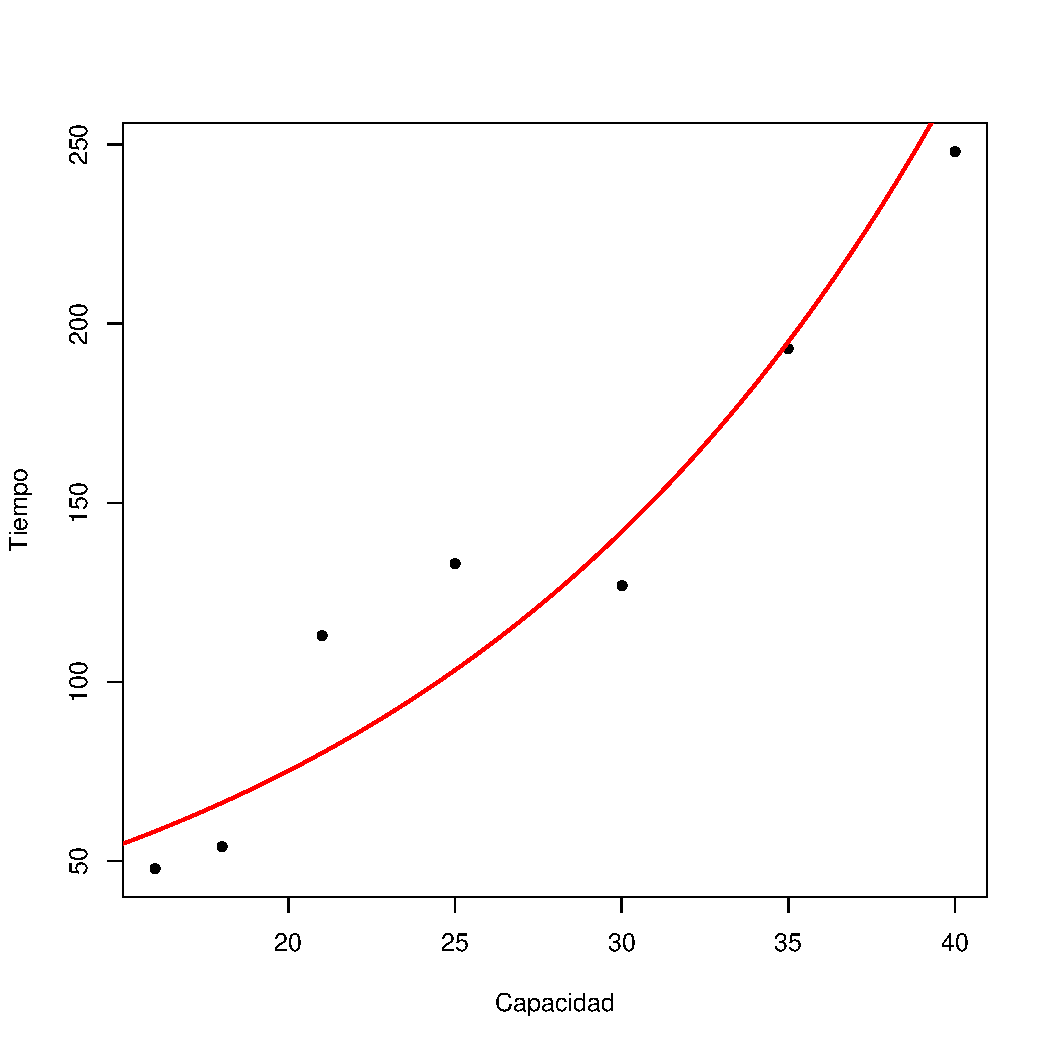
\includegraphics[width=0.7\textwidth,height=\textheight,keepaspectratio]{capacity_time.pdf}
    \caption{Comportamiento de tiempo según los monomios}
    \label{fig:time}
\end{figure}

\section{\textit{CPU vs. GPU}}

Ahora, teniendo dos versiones de la misma porción del algoritmo, una secuencial y otra en paralelo, solo quedaría ver cuál de las dos tiene mejor desempeño. Se realizaron varias pruebas en este punto, ajustando los parámetros de configuración para obtener los mejores resultados. Sorprendentemente, el tiempo de ejecución para la versión \textit{GPU} resulta tener un desempeño ligeramente peor. Esto puede deberse a varias cosas, entre ellas: la tarjeta gráfica utilizada, carga computacional para delegar tareas y recoger resultados o delegación de cómputos muy sencillos; las mismas se describen a continuación.

\subsection{Procesamiento limitado de la \textit{GPU}}

La \textit{GPU} disponible no tiene las mejores especificaciones para realizar pruebas que requieran múltiples cómputos. Dado que existe una relación entre el tipo de tarea que se le delegue a la \textit{GPU}, y la forma como son asignados estos pequeños trabajos, con la cantidad de unidades de cómputo que tenga el dispositivo.

\subsection{Delegar trabrajo tiene su precio}

Crear un contexto, cola de comandos, establecer los parámetros de una función \textit{kernel} y ejecutar ese programa tiene un costo en términos de tiempo. Por lo que sería conveniente asignar tareas que requieran más trabajo por parte de cada unidad del dispositivo. También puede incrementarse el número de trabajos delegados, cambiando la estrategia de paralelismo, pero la \textit{GPU} sigue sin tener grandes capacidades.

\subsubsection{Asignación de tareas}

En OpenCL existe un parámetro para indicar el número de elementos con los que trabajará cada unidad, es decir, cómo se distribuye el trabajo total. Por ejemplo, si se indica que cada unidad va a trabajar con una tarea a la vez del total, y este total es mayor que el número de unidades en el dispositivo, se necesitaría esperar a que se desocupe alguna unidad para asignarle una nueva tarea. Por ello, se asginan en grupos para aprovechar toda la \textit{GPU} pero si esta es limitada, y el número total de tareas es muy grande, los recursos se ven colapsados.
\chapter{Conclusiones}

\begin{chapquote}{Radiohead, \textit{Where I End and You Begin}}
\noindent
Hay una brecha de por medio\\
Hay una brecha donde nos encontramos\\
Donde yo termino y tu empiezas\\
\\
Y lo siento por nosotros\\
Los dinosaurios vagan por la tierra\\
El cielo se vuelve verde\\
Donde yo termino y tu empiezas
\end{chapquote}

\sat es un problema de gran relevancia, que tiene la capacidad de modelar otro problema traduciendo las condiciones que lo definan a fórmulas lógicas. Con la versatilidad que posee, vale la pena invertir esfuerzos en buscar una buena solución para él, ya que será la solución a varias problemas.

Se ha presentado una perspectiva diferente al enfoque que suele tener este problema, una representación que podría tener el potencial de mejorar el rendimiento con la disponibilidad suficiente de recursos, además de su correcta utilización, aprovechando al máximo de ellos. La solución que se ha ideado es, claramente, perfectible pero como un primer acercamiento ha resultado tener resultados que dejan la posibilidad de extender, modificar y mejorar la implementación actual.

OpenCL es una plataforma que facilita el uso de la \textit{GPU} pero usarla correctamente lleva tiempo y varias pruebas para poder explotar completamente ese recurso. Los resultados obtenidos dejan acongojado a cualquiera, y sin duda esta representación puede tener otros usos, por lo que se han identificado posibles trabajos futuros que se enuncian a continuación.

\section{Trabajo futuro}

\subsection{Implementar otra estrategia para la multiplicación de polinomios}

Siendo uno de los puntos claves del algoritmo, sería conveniente continuar el trabajo enfocándose en esta operación. Existen otros métodos para multiplicar polinomios que son más eficientes, por ejemplo, a través de la transformada rápida de Fourier, pero habría que dilucidar cómo se podría adaptar al polinomio de \textit{Zhegalkin}.

\subsection{Modificar la distribución de tarea a la \textit{GPU}}

La implementación actual usa la \textit{GPU} para realizar una tarea relativamente sencilla, sería prudente implementar una función que efectúe un número mayor de operaciones y distribuya las tareas de una manera diferente. OpenCL brinda la posibilidad de usar más de una dimensión para asignar tareas a los \textit{kernels} y si hay la posibilidad de usar una tarjeta gráfica de gran capacidad, puede que exista algún aceleramiento.

\subsection{Usar una versión nuevo de OpenCL}

La versión más reciente de OpenCL es la \texttt{2.2} y existe la posibilidad de tener una implementación en \textit{C++}, por lo que sería interesante ver que nuevas caracteristicas ofrece esa nueva versión y que facilidades brindaría usar otro lenguaje de programación. Investigar cuáles serían las posibles vías de comunicación entre los \textit{kernels} para realizar tareas más complejas y aprovechar aun más la \textit{GPU}.

% \newpage

% \thispagestyle{lastpage}

% \phantom{x}
% \vfill
% \begin{chapquote}{Ethel Watts Mumford}
% \noindent Dios nos dio a nuestros familiares; gracias a Dios podemos elegir a nuestro amigos
% \end{chapquote}
% \vfill
% \phantom{x}

\end{document}